\documentclass[draft,jgrga]{agutexSI2019}


\usepackage{graphicx}
\setkeys{Gin}{draft=false}

\usepackage{xr}
\usepackage{xspace}
\usepackage{amsmath}
\usepackage{amssymb}
\usepackage{xcolor}
\usepackage{etoolbox}

\externaldocument{case_for_temperature}  % main text labels (no .tex extension)

% agutexSI2019.cls sets \@currentlabel for \section and \subsubsection from the
% raw counter instead of \thesection/\thesubsubsection, so \label targets on
% those heads lose the "S" prefix added below (\subsection is unaffected and
% already uses \thesubsection). Patch both to keep \ref{} from the main text
% reading "Sec. S2", "Sec. S2.3.1", etc.
\makeatletter
\patchcmd{\xxsection}%
  {\def\@currentlabel{\ifappendon\thesection\else\the\c@section\fi}}%
  {\def\@currentlabel{\ifappendon\thesection\else\thesection\fi}}%
  {}{\typeout{** WARNING: xxsection @currentlabel patch failed **}}
\patchcmd{\xxsubsubsection}%
  {\def\@currentlabel{\the\c@section.\the\c@subsection.\the\c@subsubsection}}%
  {\def\@currentlabel{\thesubsubsection}}%
  {}{\typeout{** WARNING: xxsubsubsection @currentlabel patch failed **}}
\makeatother

%%%%%%% MAKE SOME COMMANDS %%%%%%%%%%
\newcommand{\eqtn}[1]{Eq.~(\ref{#1})}       % Equation reference
\newcommand{\fig}[2]{\textcolor{black}{(Fig.~\ref{#1}{#2})}}   % Figure reference
\newcommand{\fignop}[2]{\textcolor{black}{Fig.~\ref{#1}{#2}}}  % Figure reference

\newcommand{\todo}[1]{\textcolor{purple}{TODO: #1}}      % Comments
\newcommand{\comment}[1]{\textcolor{cyan}{#1}}     % TODO notes
\newcommand{\mynum}[1]{\textcolor{red}{#1}}
% meteorological terms go here
\newcommand{\tmin}{\textcolor{black}{$T_{\mathrm{min}}$}\xspace}
\newcommand{\tair}{\textcolor{black}{$T_{\mathrm{air}}$}\xspace}
\newcommand{\tsfc}{\textcolor{black}{$T_{\mathrm{sfc}}$}\xspace}
\newcommand{\qair}{\textcolor{black}{$q_{\mathrm{air}}$}\xspace}
\newcommand{\qsfc}{\textcolor{black}{$q_{\mathrm{sfc}}$}\xspace}
\newcommand{\lwnet}{\textcolor{black}{$LW_{\mathrm{net}}$}\xspace}
\newcommand{\wspd}{\textcolor{black}{$w_{\mathrm{spd}}$}\xspace}
\newcommand{\wdir}{\textcolor{black}{$w_{\mathrm{dir}}$}\xspace}
\newcommand{\cloudfrac}{\textcolor{black}{$C_{\mathrm{frac}}$}\xspace}
\newcommand{\dq}{\textcolor{black}{$\Delta q$}\xspace}
\newcommand{\dT}{\textcolor{black}{$\Delta T$}\xspace}
\newcommand{\fq}{\textcolor{black}{$F\mathrm{_q}$}\xspace}
\newcommand{\ustar}{\textcolor{black}{$u_{\star}$}\xspace}
\newcommand{\lwup}{\textcolor{black}{$LW\uparrow$}\xspace}
\newcommand{\lwdn}{\textcolor{black}{$LW\downarrow$}\xspace}
\newcommand{\tsnow}{\textcolor{black}{$T_{\mathrm{snow}}$}\xspace}
\newcommand{\qsnow}{\textcolor{black}{$q_{\mathrm{snow}}$}\xspace}
\newcommand{\pbaro}{\textcolor{black}{$P_{\mathrm{baro}}$}\xspace}
\newcommand{\rnet}{\textcolor{black}{$R_{\mathrm{net}}$}\xspace}
\newcommand{\swnet}{\textcolor{black}{$SW_{\mathrm{net}}$}\xspace}
\newcommand{\swdn}{\textcolor{black}{$SW\downarrow$}\xspace}
\newcommand{\swup}{\textcolor{black}{$SW\uparrow$}\xspace}
\newcommand{\albedo}{\textcolor{black}{$\alpha$}\xspace}

% units
\newcommand{\um}{\textcolor{black}{$\mu$m}\xspace}
\newcommand{\ms}{\textcolor{black}{m$\cdot$s$^{-1}$}\xspace}
\newcommand{\gkg}{\textcolor{black}{g$\cdot$kg$^{-1}$}\xspace}
\newcommand{\kmsq}{\textcolor{black}{km$^2$}\xspace}  % kilometers
\newcommand{\wmsq}{\textcolor{black}{W$\cdot$m$^{-2}$}\xspace}
\newcommand{\degr}{\textcolor{black}{$^\circ$}\xspace}
\newcommand{\degrc}{\textcolor{black}{$^\circ$C}\xspace}
\newcommand{\gmtwo}{\textcolor{black}{gm$^{-2}$}\xspace}
\newcommand{\kgmtwo}{\textcolor{black}{kg$\cdot$m$^{-2}$}\xspace}

% prefix section/equation counters with S so cross-references from the main text read Sec. S2.1, Eq. S1
% (\thefigure and \thetable already carry an "S" prefix by default in agutexSI2019.cls)
\renewcommand{\thesection}{S\arabic{section}}
\renewcommand{\theequation}{S\arabic{equation}}

\begin{document}

\title{Supporting Information for "Solar radiation primarily drives snow ablation during the March 2026 heat wave in the California Sierra Nevada"}

\authors{William Rudisill\affil{1}, Alan Rhoades\affil{1}, Megan Mason\affil{2}, Gabriel Lewis\affil{2}, Andrew Schwartz\affil{2}, Marianne Cowherd\affil{4}, Benjamin Hatchett\affil{3}, Erica Siirila-Woodburn\affil{1}, Dan Feldman\affil{1}}

\affiliation{1}{Lawrence Berkeley National Laboratory, Earth and Environmental Sciences Area}
\affiliation{2}{UC Berkeley Central Sierra Snow Laboratory}
\affiliation{3}{Colorado State University}
\affiliation{4}{Montana State University}

\begin{article}

\noindent\textbf{Contents of this file}
\begin{enumerate}
\item Text S1 to S3
\item Figures S1 to S9
\end{enumerate}

\section{Snow covered area and streamflow anomalies}
To investigate the hydrologic ramifications of early snow ablation in 2026, we obtained streamflow data from the USGS Sagehen Creek gage, which has long-term records and drains into the Truckee river watershed, one watershed to the east of CSSL. 
We find that the monthly average streamflow at the Sagehen Creek site peaked in March, two months earlier than normal (Fig.~\ref{fig:supp_sagehen_q}), and reached flows well above those typical for March.

The regional pattern of snow-covered area change also reveals the extent of the anomalous March.
The SPIReS snow-covered area (SCA) product shows the lowest SCA on record (Fig.~\ref{fig:supp_scachange}).
SCA was already very low leading up to March, but reached even lower levels by 31 March.
High-elevation regions above 2250 m had nearly 100\% SCA prior to the March event, but those regions also declined substantially.

\section{SUMMA details}\label{supp:summa_details}
%% Sensible and Latent heat fluxes
This section describes assumptions implicit in SUMMA and provides additional details about the model forcing data preparation.
\subsection{Model flux equations}\label{supp:summa_desc_model_eq}

The bulk expression for $H_s$ implemented in SUMMA is given by:

\begin{align}
H_s &=  c_p \rho C_h u (T_{\mathrm{air}} - T_{\mathrm{snow}}) \label{eq:supp_bulk2},
\end{align}

where $c_p$ is the specific heat capacity of dry air (constant), $u$ is the horizontal wind speed, $\rho$ is the dry air density, and $C_h$ is the bulk transport coefficient.
In this work, we use the SUMMA formulation for $C_h$, which models the stability correction as a function of the bulk Richardson number.
We use the ``Louisinv'' stability correction function implemented in the SUMMA model and assume that $z_h = z_0$:
\begin{equation}
C_h = \frac{k^2}{[\ln(z/z_0)]^2}\cdot f(\mathrm{Ri}),
\end{equation}
where $k$ is the von K\'arm\'an constant, $z$ is the measurement height, $z_0$ is the roughness length, and Ri is the bulk Richardson number, defined as
\begin{equation} \label{eq:ri}
    \mathrm{Ri}(z) = \frac{g\, z\, (T_{\mathrm{air}} - T_{\mathrm{snow}})}{0.5(T_{\mathrm{air}} + T_{\mathrm{snow}})\, u^2},
\end{equation}
and $f(\mathrm{Ri})$ is a function with range (0,1] that declines with increasing Ri.
An equivalent formulation for latent heat flux follows Eq.~\ref{eq:supp_bulk2}.
The stability correction is reproduced and used in Fig.~\ref{fig:idealized_sens_heat} of the main text.
The $f(\mathrm{Ri})$ used in that figure is given by $f(\mathrm{Ri}) = (1 - 5\,\mathrm{Ri})^{-2}$.

% #$1/(1 + \tfrac{b}{2}\mathrm{Ri})^2$

\subsection{Forcing data}
We use bias-corrected ERA5 data as forcing for SUMMA, with several key processing steps.
ERA5 data were obtained from the Copernicus data store for the grid cell nearest CSSL.
\swdn was compared between ERA5 and the CSSL CNR4 radiometers for water year 2026.
We developed a correction factor to account for potential shadowing by canopy adjacent to the site, using solar zenith angle (SZA) and solar azimuth angle (AZM) as predictors.
These were computed using the Python PyEphem package.
The correction grid is depicted in Fig.~\ref{fig:supp_fig_SWd_adjust_sza_azm}.
It shows the multiplicative correction between 0 and 1 for each SZA and AZM.



\clearpage

\subsection{Additional SUMMA model outputs and model validation}\label{supp:sec:validation}
Additional SUMMA outputs with relevance to interpreting the main text are displayed in this section, as well as additional model validation plots.

The snowpack accumulated substantial liquid water following the February ROS event, and snow temperatures were nearly isothermal (Fig.~\ref{fig:supp_twod_vert_plots_ice_liq_dens_temp}).
Cold-content generation began during March in a thin layer at the top of the snowpack, where liquid water also refroze.
A dense ice layer formed during mid-February and remained buried under the late-February snow and rain.


\subsubsection{Canopy site}\label{supp:sec:validation:canopy}

We validate the SUMMA model in several ways.
First, we evaluate the canopy radiation parameterization against the CSSL sub-canopy Kipp and Zonen SP Lite2 radiometer.
We find good correlation for March 2026 for the UEB 2-stream parameterization and an LAI value of 1.5 (Fig.~\ref{fig:supp_sw_validation}), using the aforementioned \swdn forcing as the top boundary condition to the model.

\clearpage




\subsubsection{Fluxes}\label{supp:sec:validation:fluxes}
CSSL hosts an experimental eddy-covariance instrument on a movable arm above the snowpack.
Eddy-covariance fluxes were processed using the LI-COR EddyPro v7.0.9 software with despiking, double coordinate rotation, and flux quality assignment.
A qualitative comparison between the SUMMA and eddy-covariance fluxes of sensible and latent heat shows reasonable agreement (Fig.~\ref{fig:supp_ecor_validation}), though there were many low-quality flux measurements during the month of March.
Key periods of sublimation during the first and last portions of the month show reasonable agreement.



\subsubsection{Albedo}\label{supp:sec:albedo}
SUMMA-modeled albedo is compared against available observations from the CSSL CNR4 radiometers, as well as SPIReS remote-sensing-based albedo (Fig.~\ref{fig:supp_albedo_validation}).


\section{Initial condition experiments}\label{supp:init_cond}
As we have shown, anomalous conditions also preceded the March 2026 ablation event.
To interrogate the role of antecedent conditions, we performed initial condition experiments by altering the amount of ice, liquid water, and cold-content.

The first test (Test 1) evaluates the effects of initial liquid water content \fig{fig:supp_initial_cond_sens1}{}.
It was constructed as follows.
The first run is the natural starting condition (liq=1).
Then, we halved the amount of liquid water (liq=0.5) and increased the amount of ice to keep the total SWE (the sum of liquid and ice water equivalent) approximately constant.
The third run completely zeros out liquid water (liq=0) and likewise increases the amount of ice to keep SWE constant.
For internal consistency in SUMMA, the layer temperature is also reduced in the zero-liquid-water case (to prevent refreezing), which yields the higher starting CC for that case \fig{fig:supp_initial_cond_sens1}{a}.
The outcomes show minimal sensitivity in the timing and rate of SWE change; the all-ice case completely ablated about one day later than the standard case.


The second test (Test 2) evaluates the effects of initial snow mass on $\Delta$SWE across the March heat wave \fig{fig:supp_initial_cond_sens2}{}.
It is composed of four model runs (SWEx1, SWEx1.5, SWEx2, and SWEx3) and uses a dry starting snow case for all experiments.
The initial dry-SWE amount is multiplied by 1, 1.5, 2, and 3, respectively.
The snow height is also adjusted to maintain an approximately uniform bulk density between the experiments \fig{fig:supp_initial_cond_sens2}{a}.
The surface temperature was assigned the same starting value in each run and decays exponentially to 0\degrc at the bottom of the snow layer.
\fignop{fig:supp_initial_cond_sens2}{b} may be interpreted as follows.
First, $\Delta$SWE is equivalent to $\Delta$Ice plus $\Delta$Liquid integrated throughout the depth of the snowpack (middle columns of \fignop{fig:supp_initial_cond_sens2}{b}).
These terms are also equivalent to the cumulative fluxes at the snowpack top/bottom boundaries, namely precipitation, sublimation/frost, and liquid water outflow through the bottom of the snowpack (rightmost columns of \fignop{fig:supp_initial_cond_sens2}{b}).

The results of this experiment show that nearly the same amount of ice melts across all scenarios ($\Delta$Ice), save for the SWEx1 case, which is limited by the amount of ice available to ablate.
However, $\Delta$SWE for the SWEx3 experiment is $-449$ mm compared to $-498$ mm for the SWEx1.5 experiment.
This discrepancy is due to the amount of liquid water retained in the snowpack ($+70$ vs. $+12$ mm for SWEx3 vs. SWEx1.5, respectively).
In this way, we can see that there is not always a 1:1 relationship between the snow energy balance and $\Delta$SWE; the residual holding capacity of snow liquid means that two snowpacks can undergo a nearly identical energy forcing, but the deeper snowpack may retain more SWE in the form of liquid water.




\clearpage



\end{article}
\clearpage

% ---------------------------------------------------------------------------
% Figures
% ---------------------------------------------------------------------------

\begin{figure}[htbp]
  \centering
  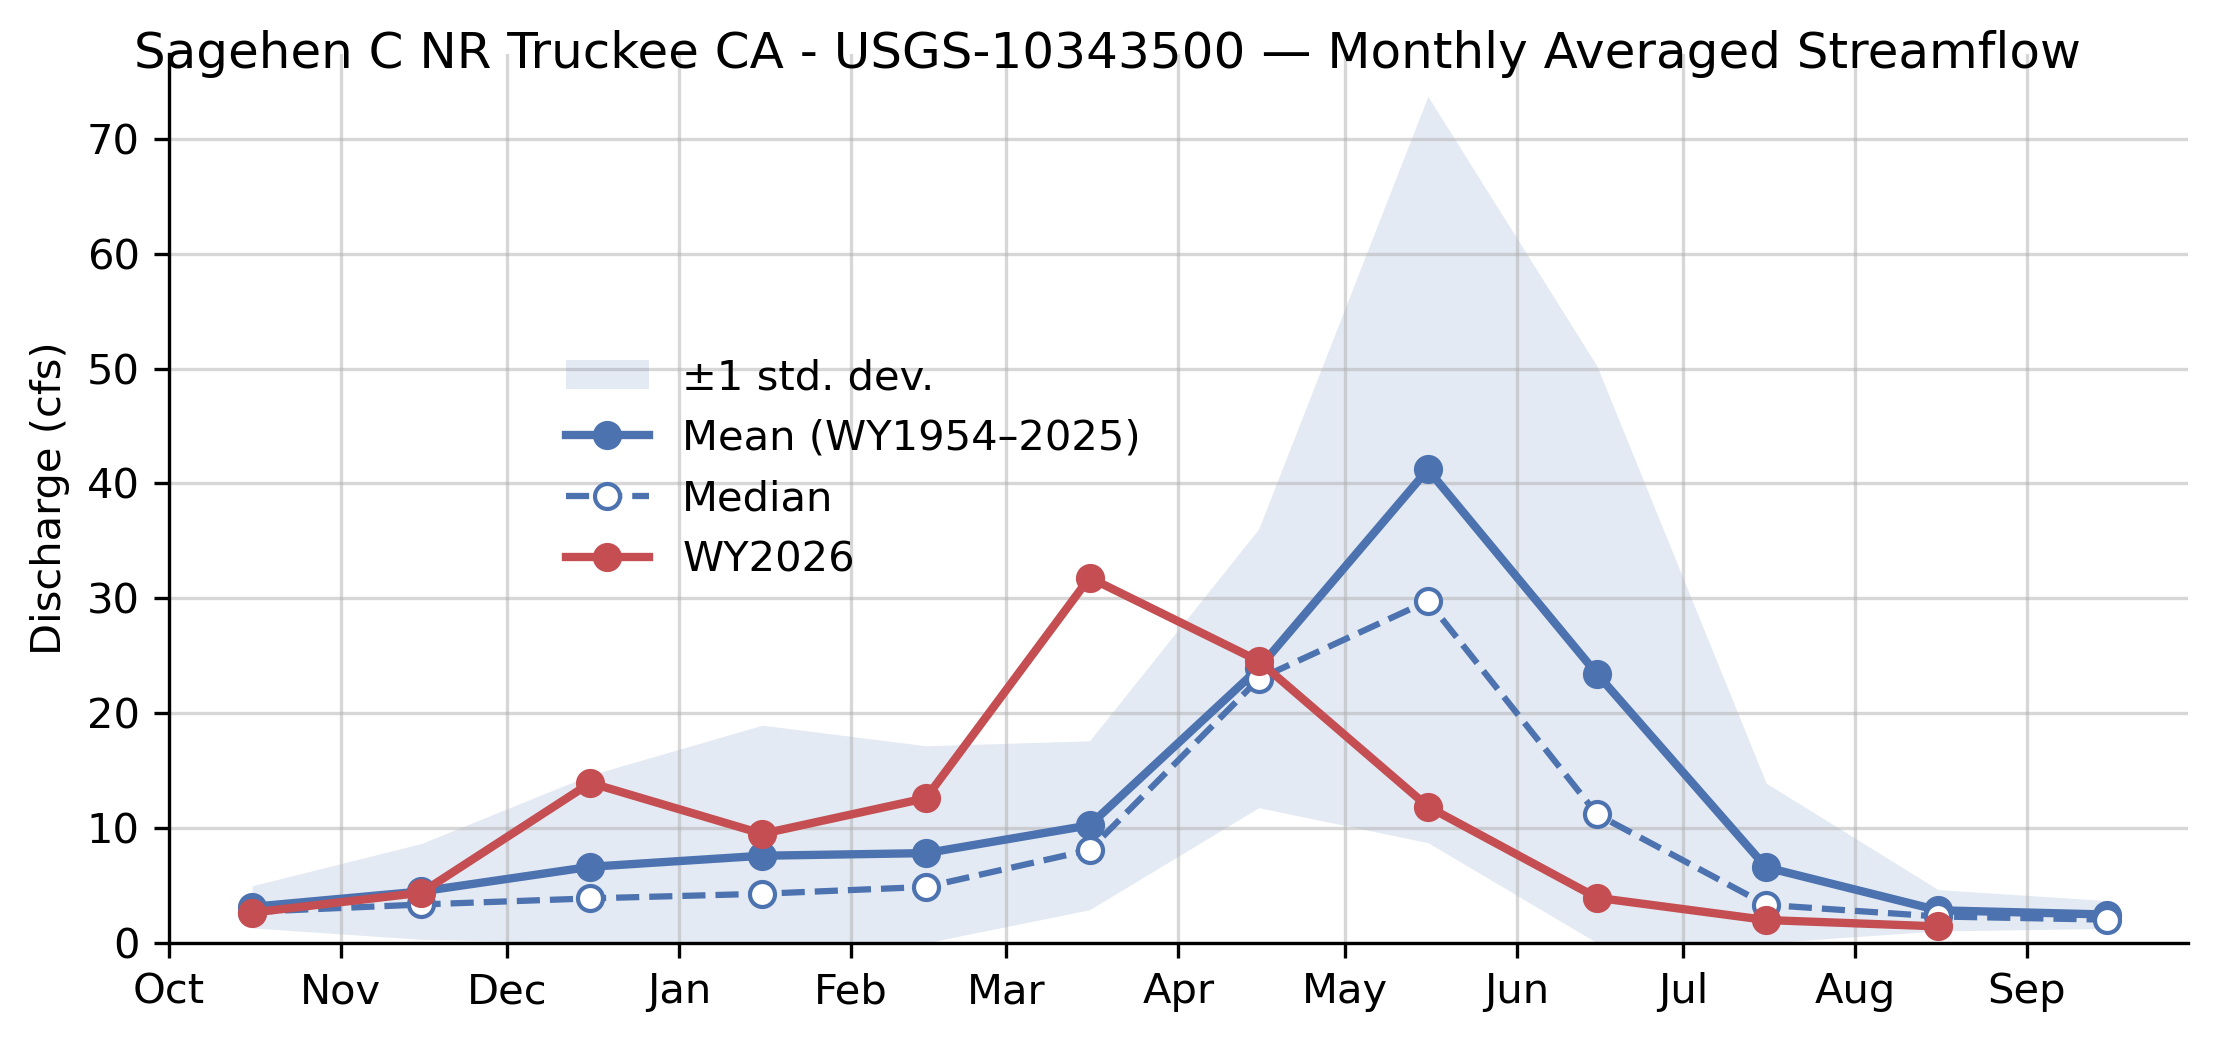
\includegraphics{images2/supp_sagehen_q.png}
  \caption{Monthly averaged streamflow in cubic feet per second (cfs) from 1954 to present for the USGS Sagehen Creek gage site.
  The historical mean, historical median, historical 1-$\sigma$ range (shaded region), and WY2026 streamflow are depicted.
  }
  \label{fig:supp_sagehen_q}
\end{figure}

\begin{figure}[htbp]
  \centering
  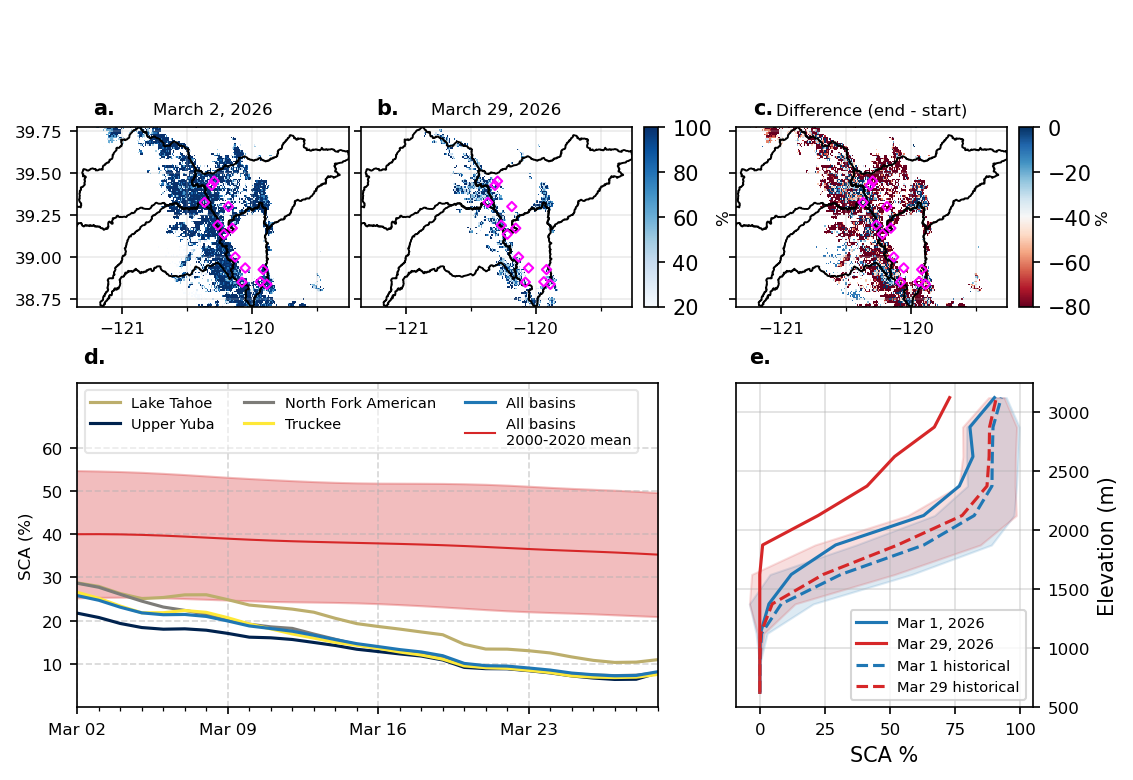
\includegraphics[width=0.8\linewidth]{images/sca_combined.png}
  \caption{SPIReS SCA across the study region during the March heat wave.
  Watershed boundaries are shown in black and SNOTEL monitoring sites are indicated by magenta diamonds.
  \textbf{(a, b, c)} SCA (\%) on March 2 and March 29, 2026, respectively, and the difference between the two dates.
  \textbf{(d)} Daily mean SCA (\%) for each individual watershed and aggregated across all four HUC8 basins (the Truckee River watershed comprises the Lake Tahoe and Truckee River HUC8 basins).
  The 2000--2020 historical mean and $\pm$1-$\sigma$ range are depicted.
  \textbf{(e)} Mean SCA as a function of elevation band (250~m bins) for March 2 (blue) and March 29 (red), shown alongside historical values for the same dates (dashed lines) with $\pm$1-$\sigma$ shading.}
  \label{fig:supp_scachange}
\end{figure}

\begin{figure}[htbp]
  \centering
  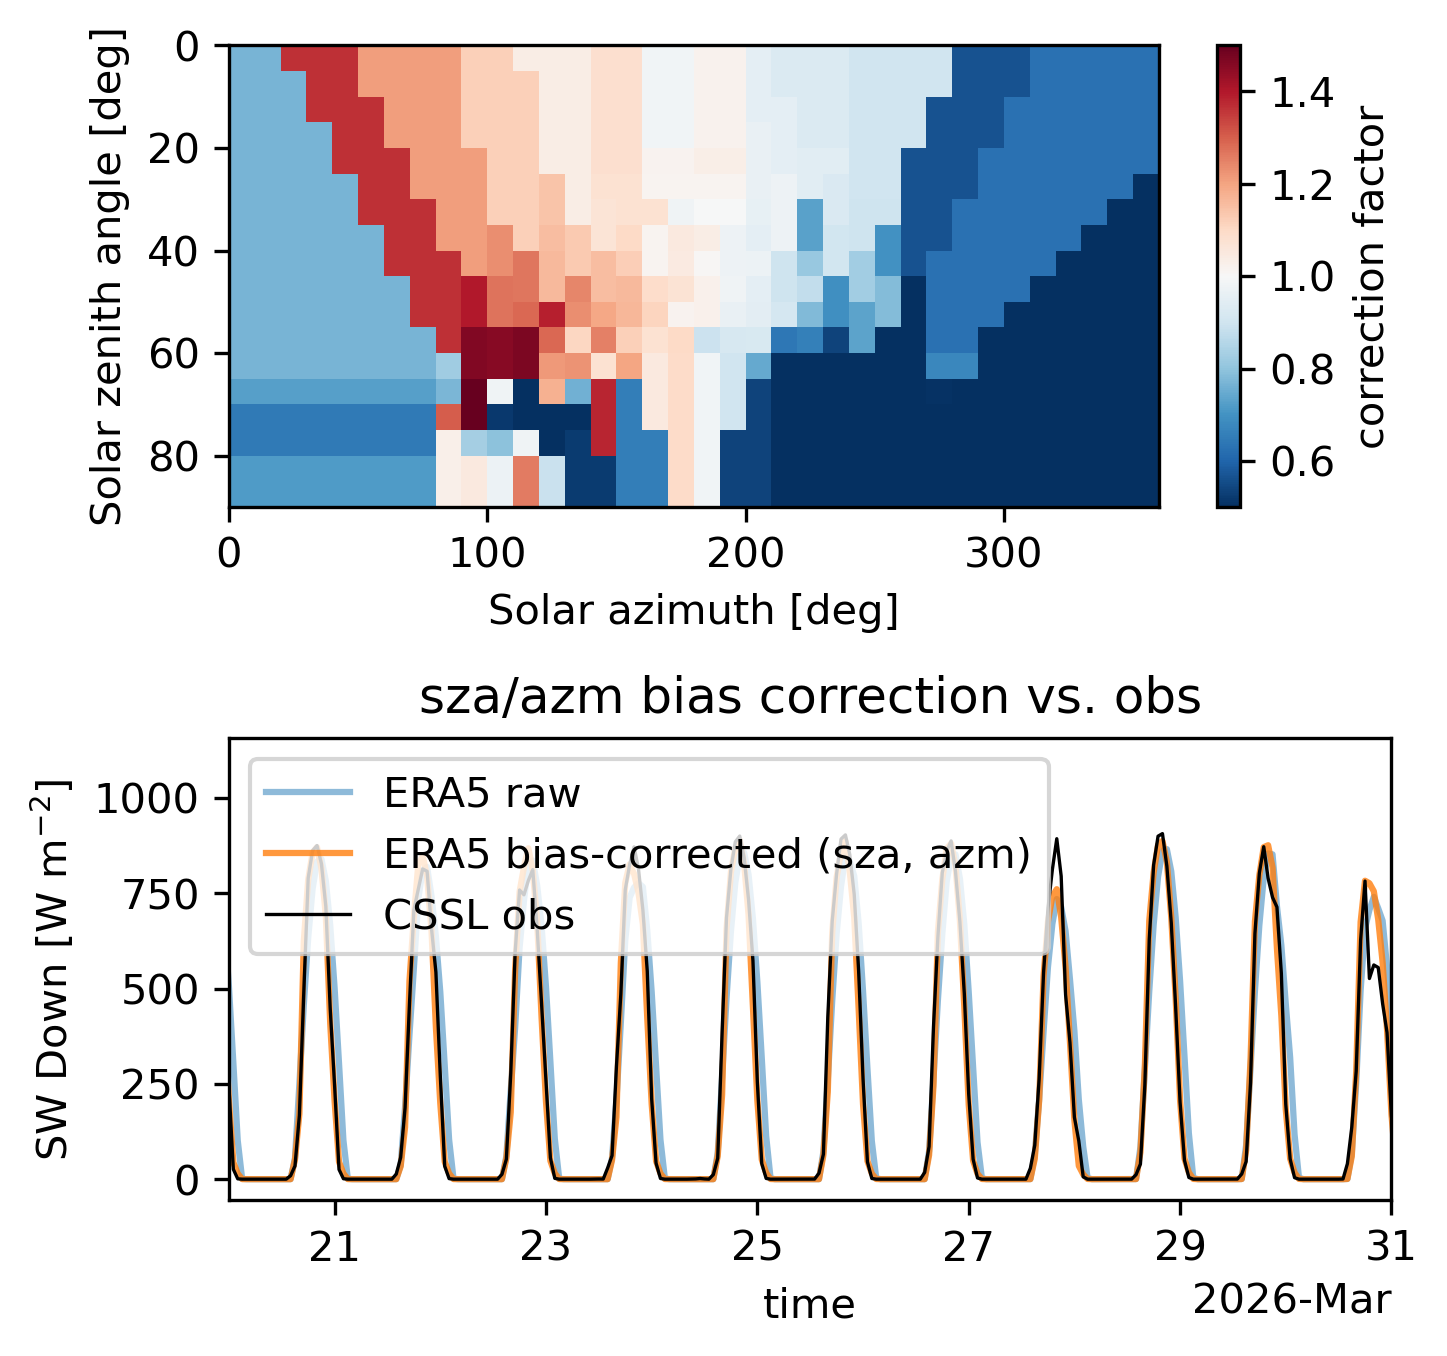
\includegraphics{images2/supp_fig_SWd_adjust_sza_azm.png}
  \caption{\swdn multiplicative correction factors for the ERA5 radiation data.
  The top plot shows the correction grid.
  The bottom plot shows the observed, uncorrected, and corrected data.
  }
  \label{fig:supp_fig_SWd_adjust_sza_azm}
\end{figure}

\begin{figure}[htbp]
  \centering
  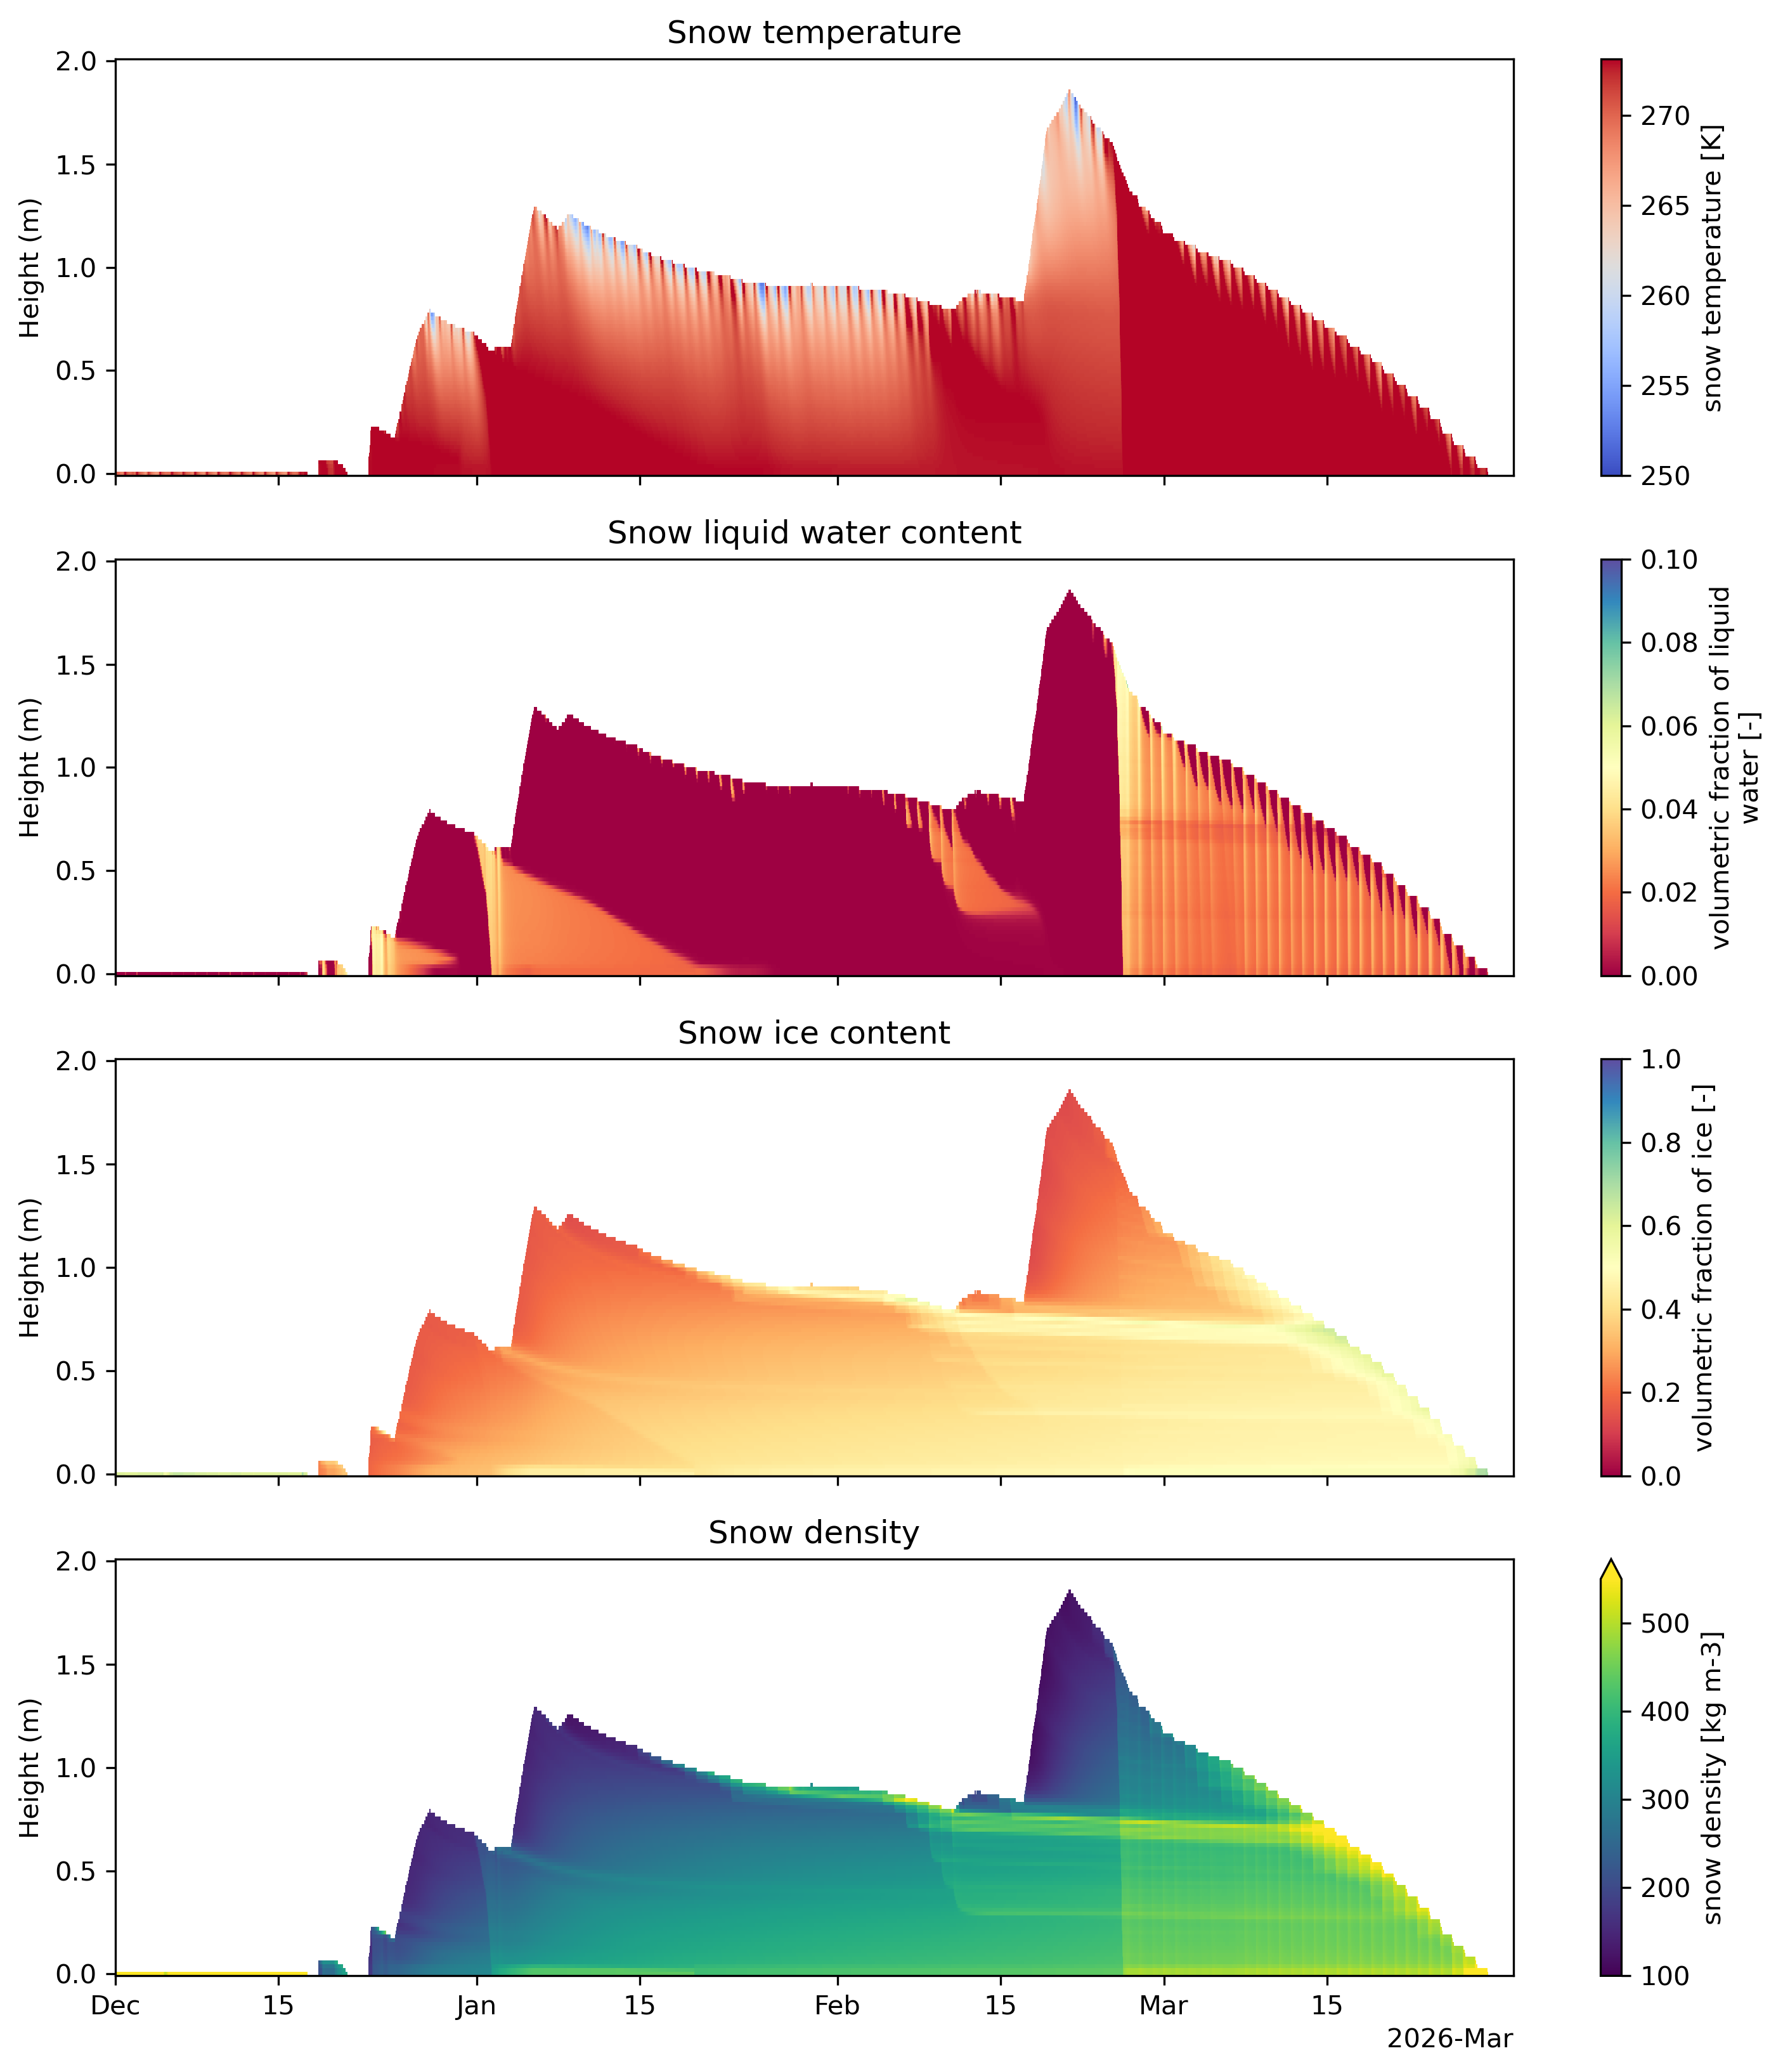
\includegraphics[width=\linewidth]{images2/supp_snowt_liq_ice_dens.png}
  \caption{A timeseries of modeled vertical cross-sections of snow temperature, snow liquid water content volumetric fraction, snow ice content volumetric fraction, and snow density (bottom) during the snow season of WY2026 for the open site at CSSL.}
  \label{fig:supp_twod_vert_plots_ice_liq_dens_temp}
\end{figure}

\begin{figure}[htbp]
  \centering
  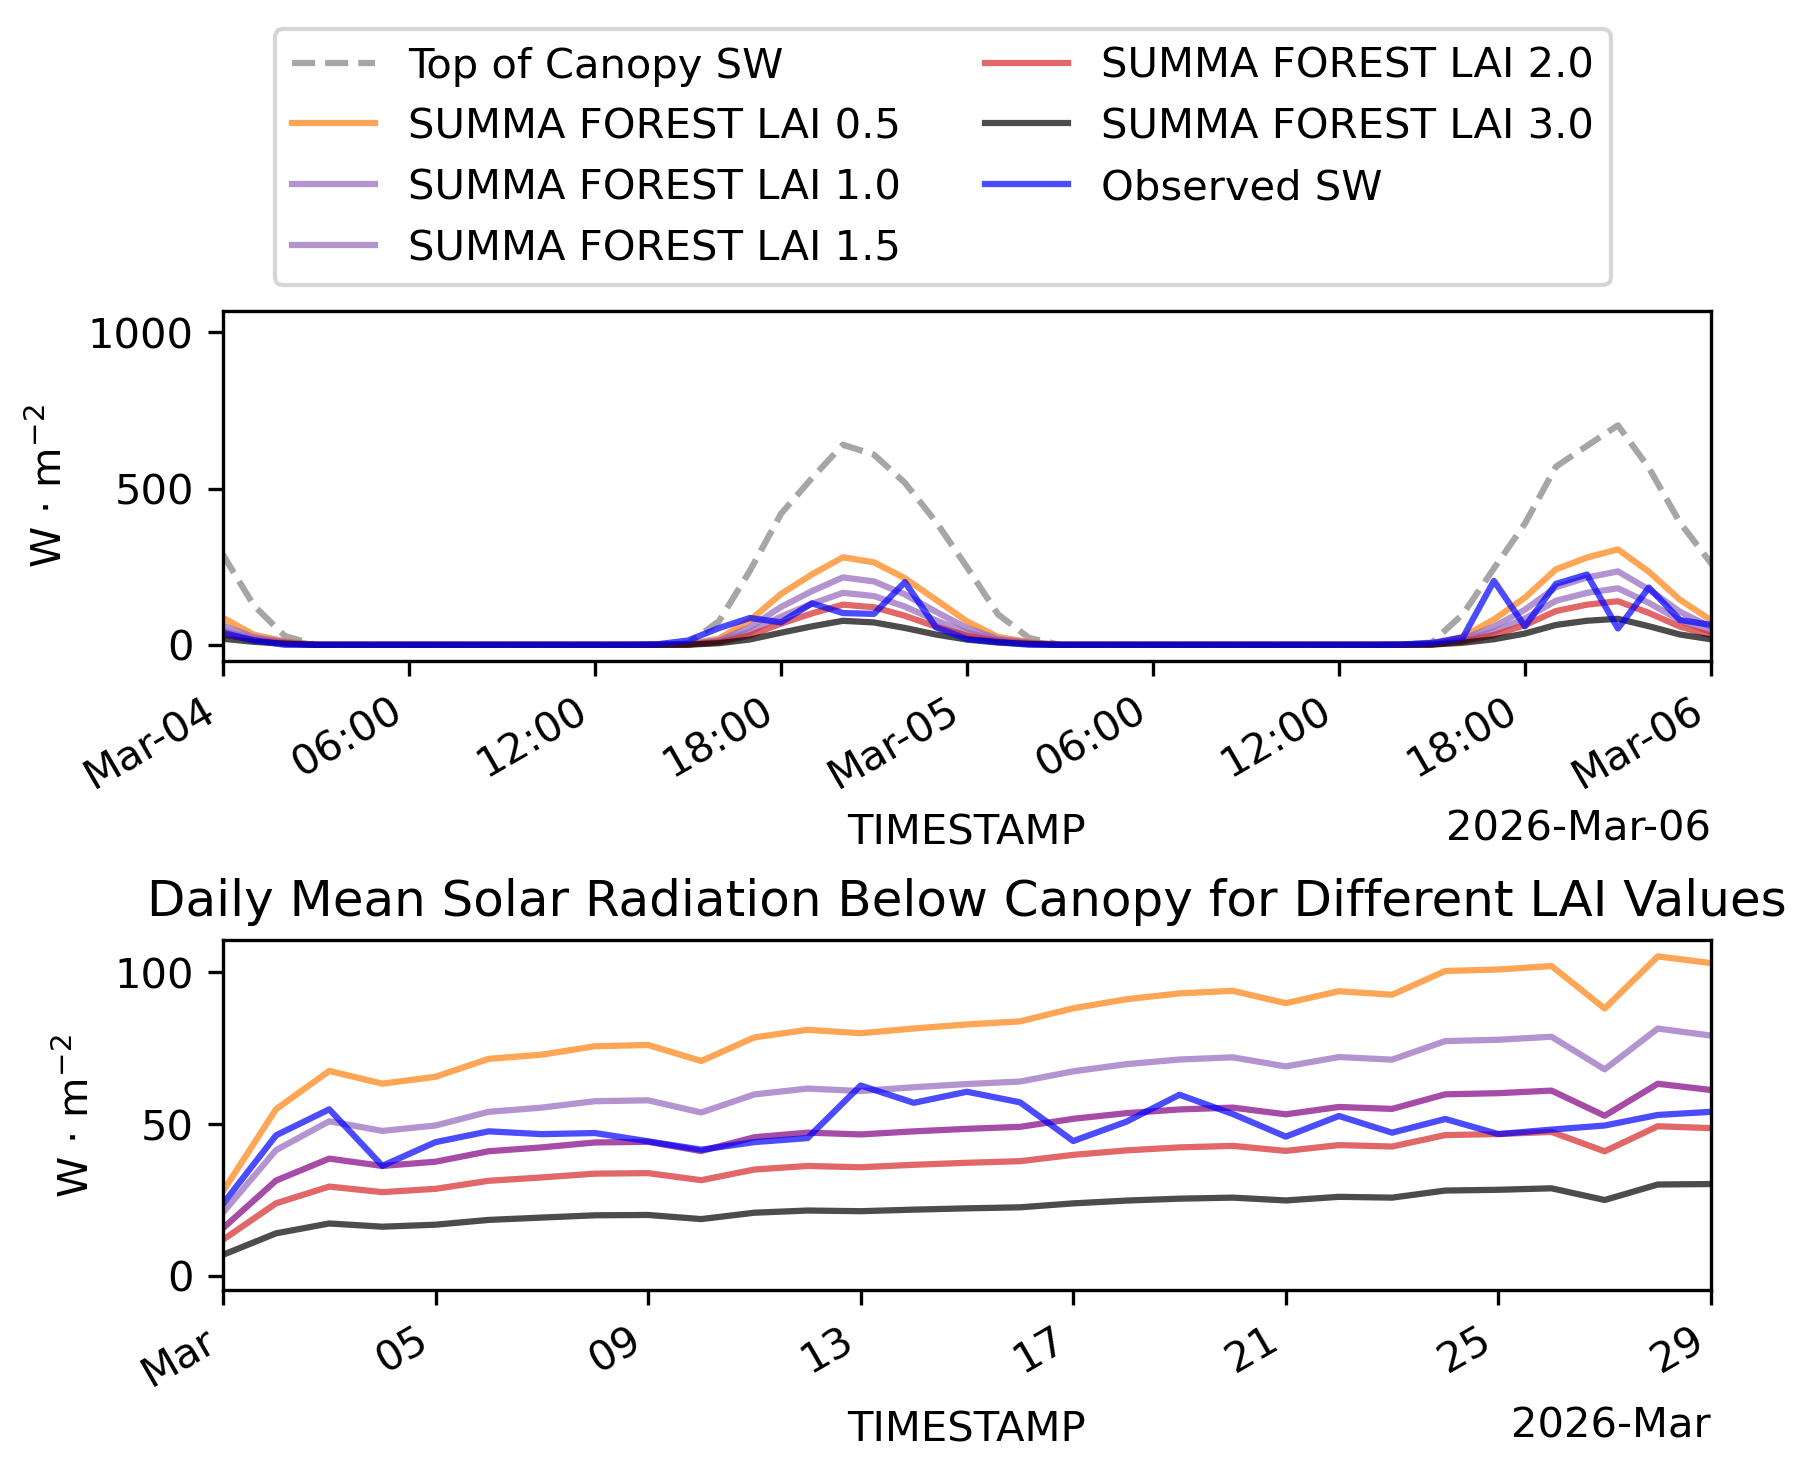
\includegraphics{images2/supp_sw_validation.png}
  \caption{A comparison of sub-canopy downwelling radiation for different LAI values using the UEB-2stream shortwave radiation parameterization.
  The top plot depicts hourly \swdn over a two-day period in early March.
  The bottom plot depicts hourly \swdn during March.
  Radiation observed by the Kipp and Zonen radiometer is depicted by the blue solid line.}
  \label{fig:supp_sw_validation}
\end{figure}

\begin{figure}[htbp]
  \centering
  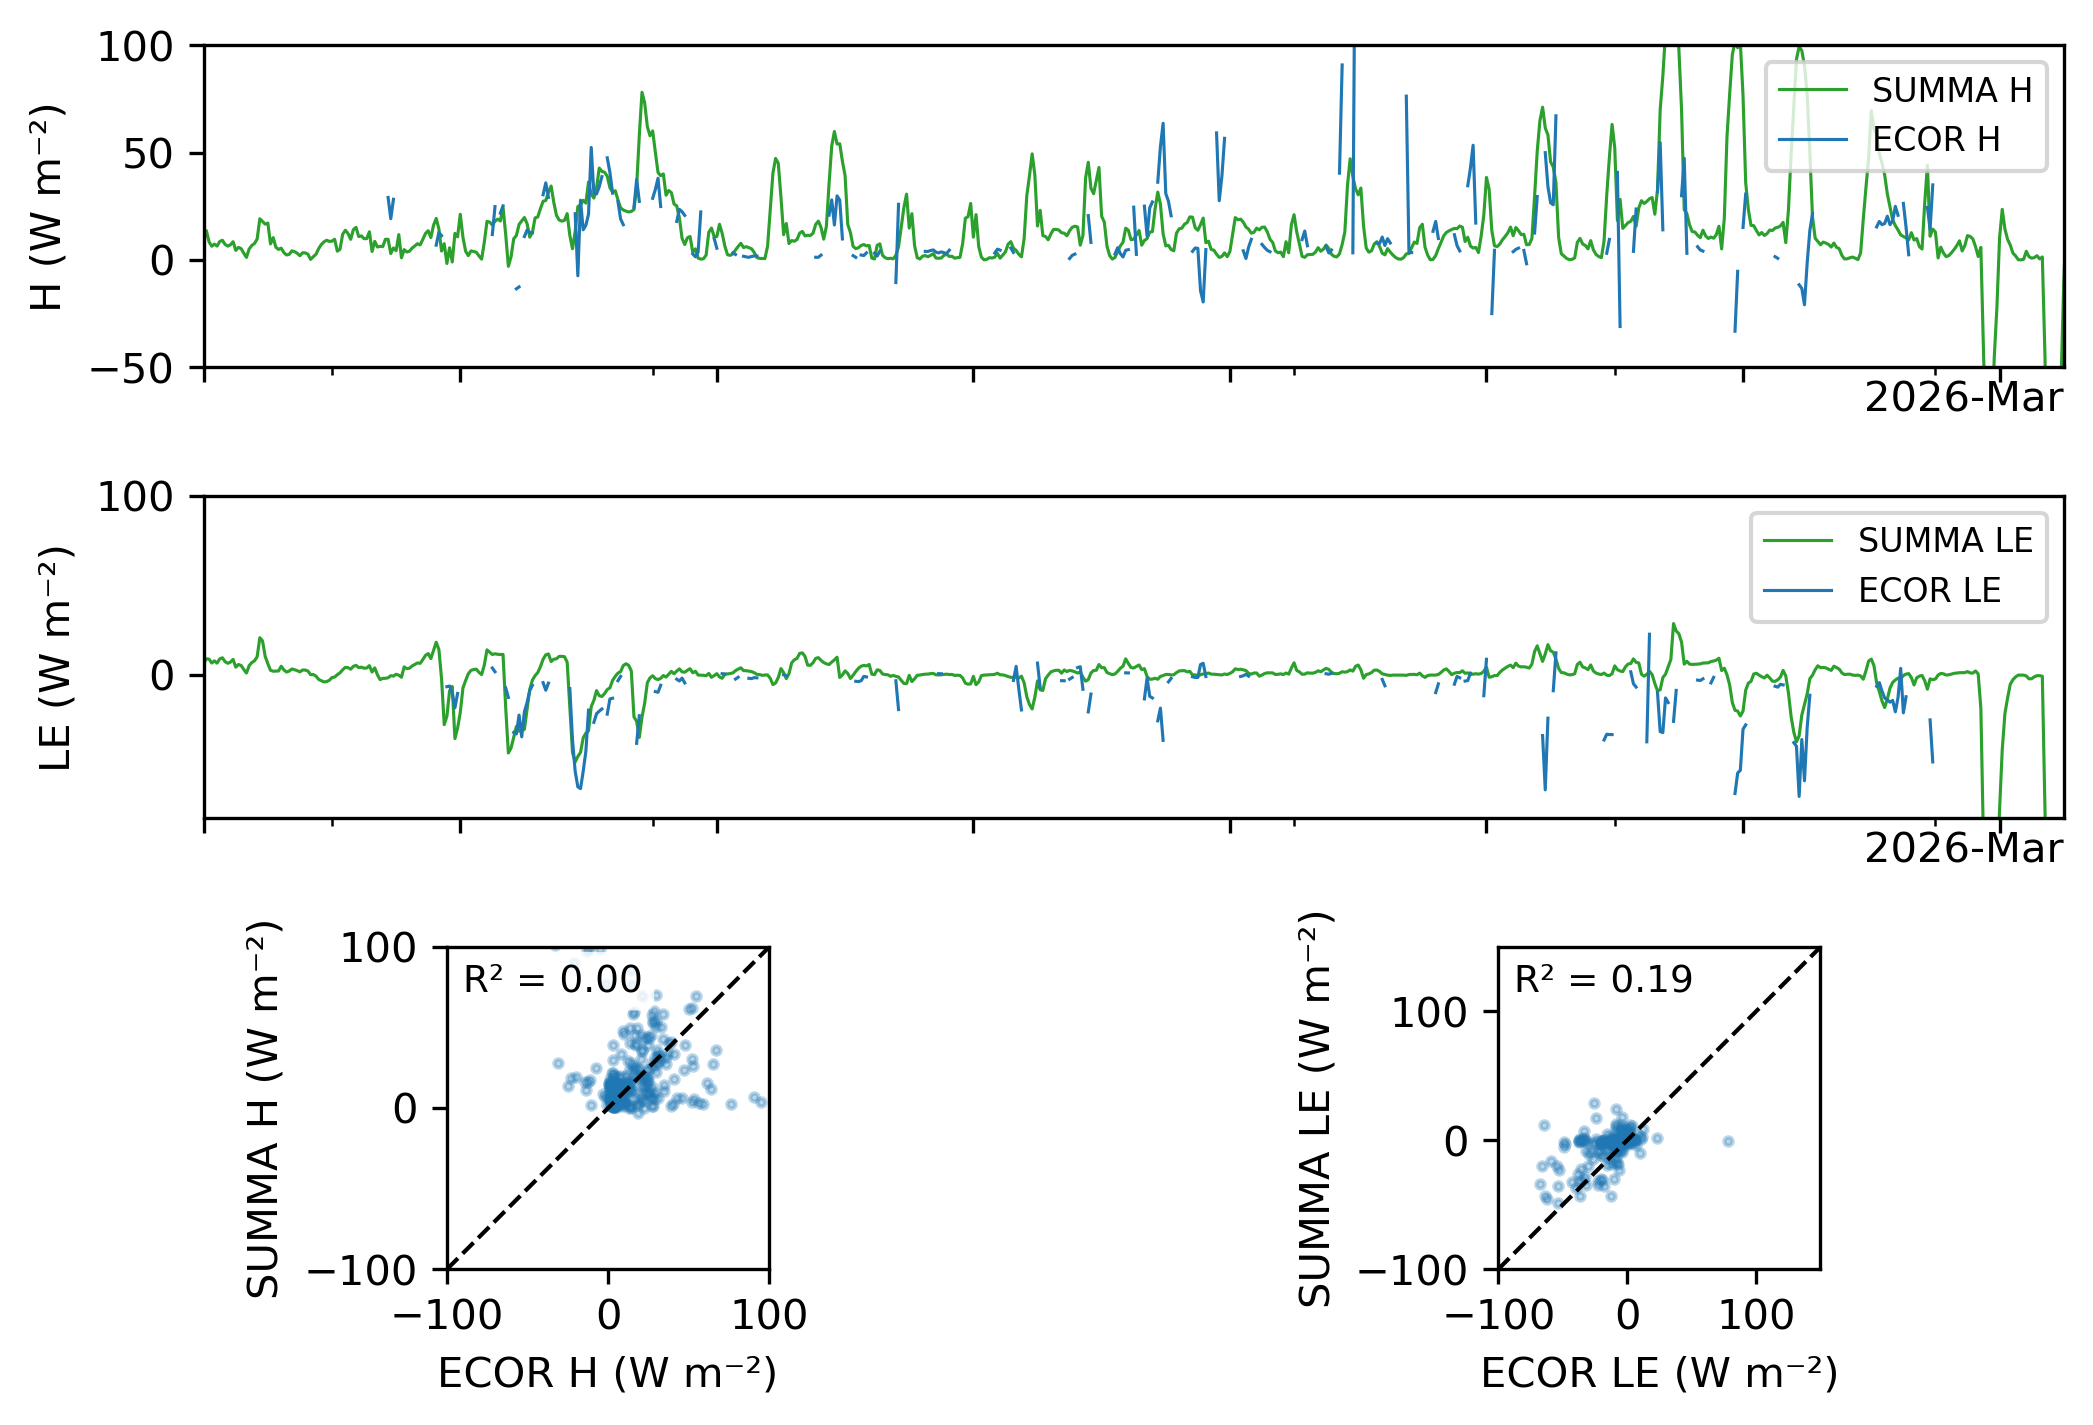
\includegraphics{images2/supp_ecor_valid.png}
  \caption{A comparison of SUMMA and eddy-covariance (ECOR) measured fluxes at CSSL for sensible heat (H) and latent heat (LE).
  The top shows a timeseries for the month of March 2026.
  The bottom two plots show 1:1 plots between the ECOR and SUMMA estimated fluxes.
  }
  \label{fig:supp_ecor_validation}
\end{figure}

\begin{figure}[htbp]
  \centering
  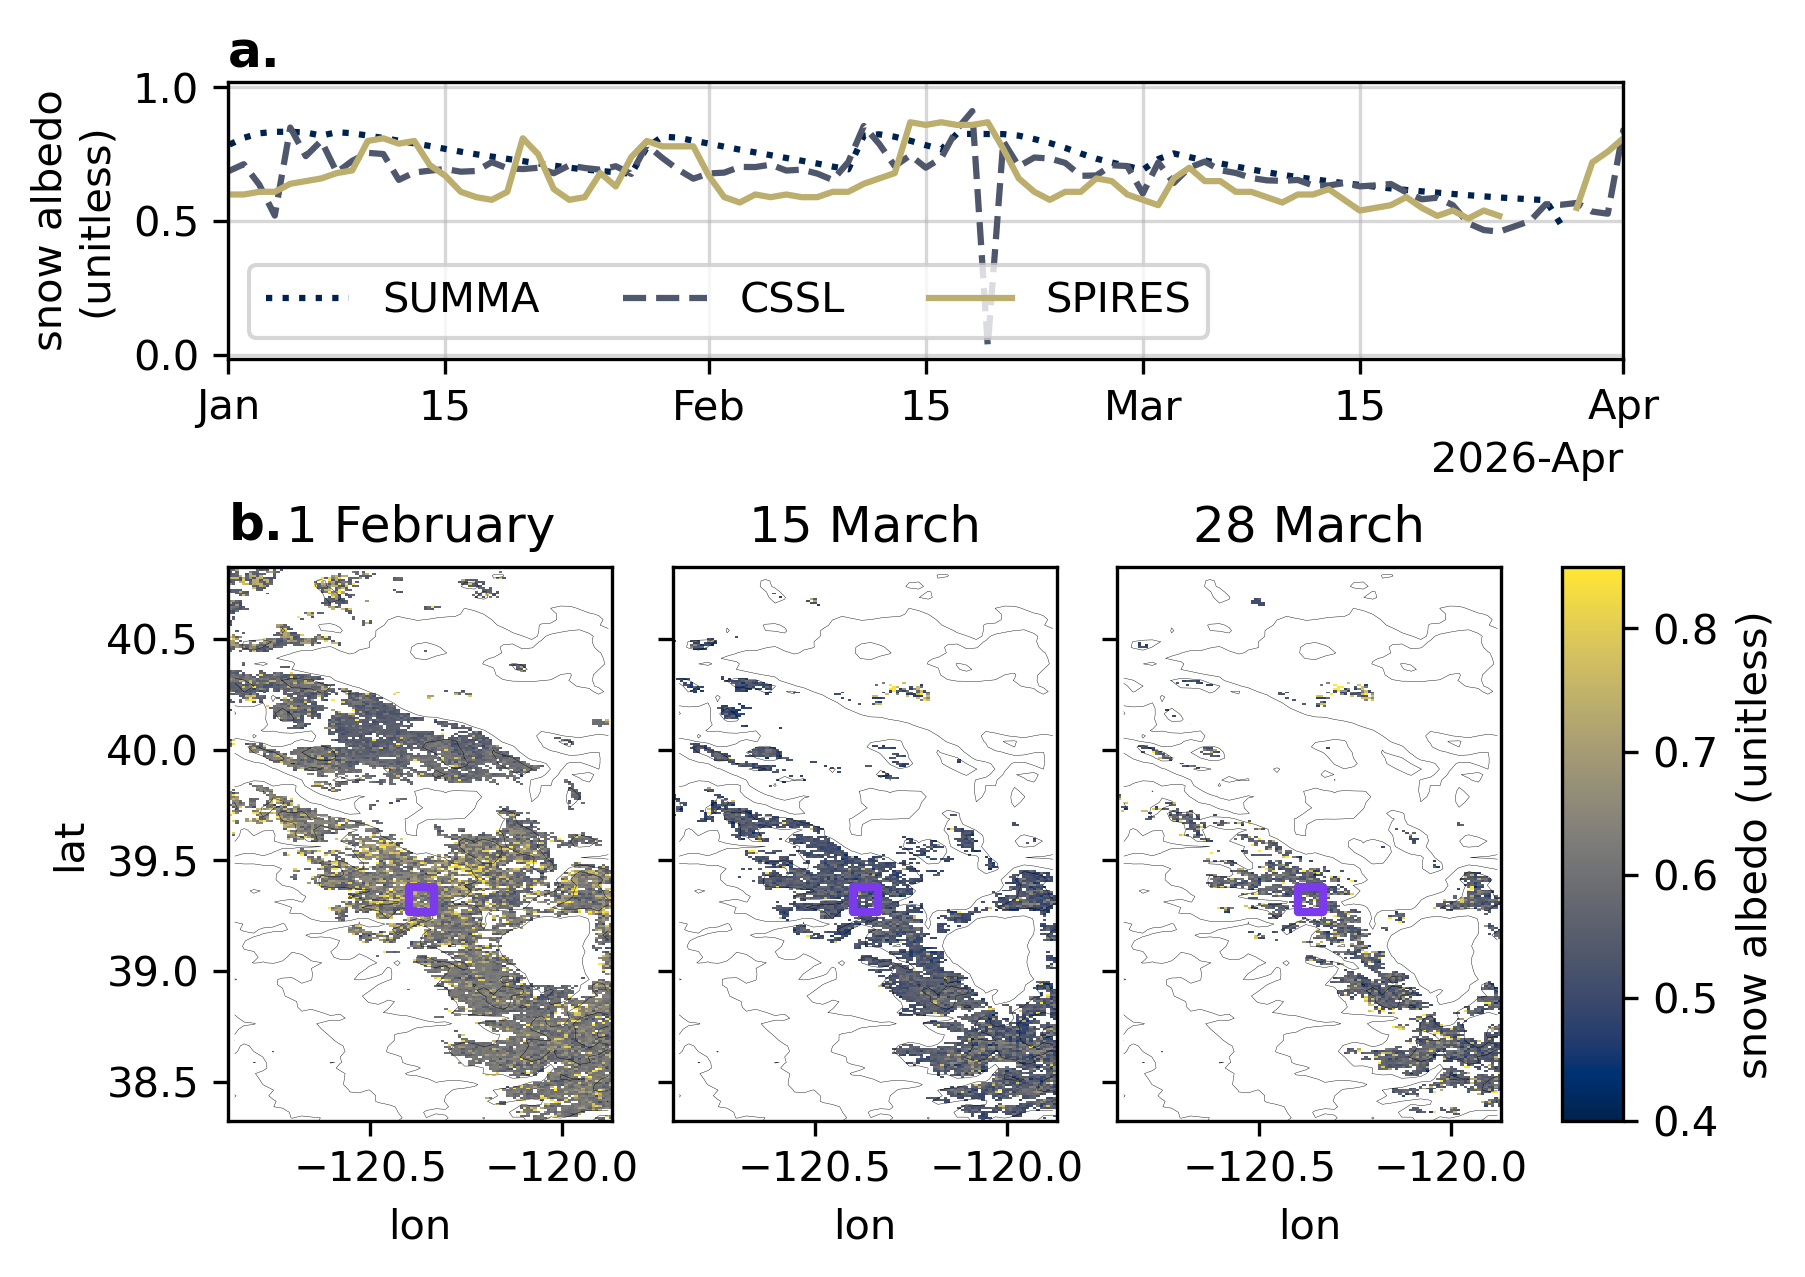
\includegraphics{images2/supp_albedo_validation.png}
  \caption{(a) SUMMA albedo evaluated against CSSL and SPIReS observations from 1 January 2026 to 1 April 2026. (b) Example maps of SPIReS snow albedo during water year 2026. CSSL is highlighted with the purple box. 500 m elevation contours are depicted for reference.}
  \label{fig:supp_albedo_validation}
\end{figure}

\begin{figure}[htbp]
  \centering
  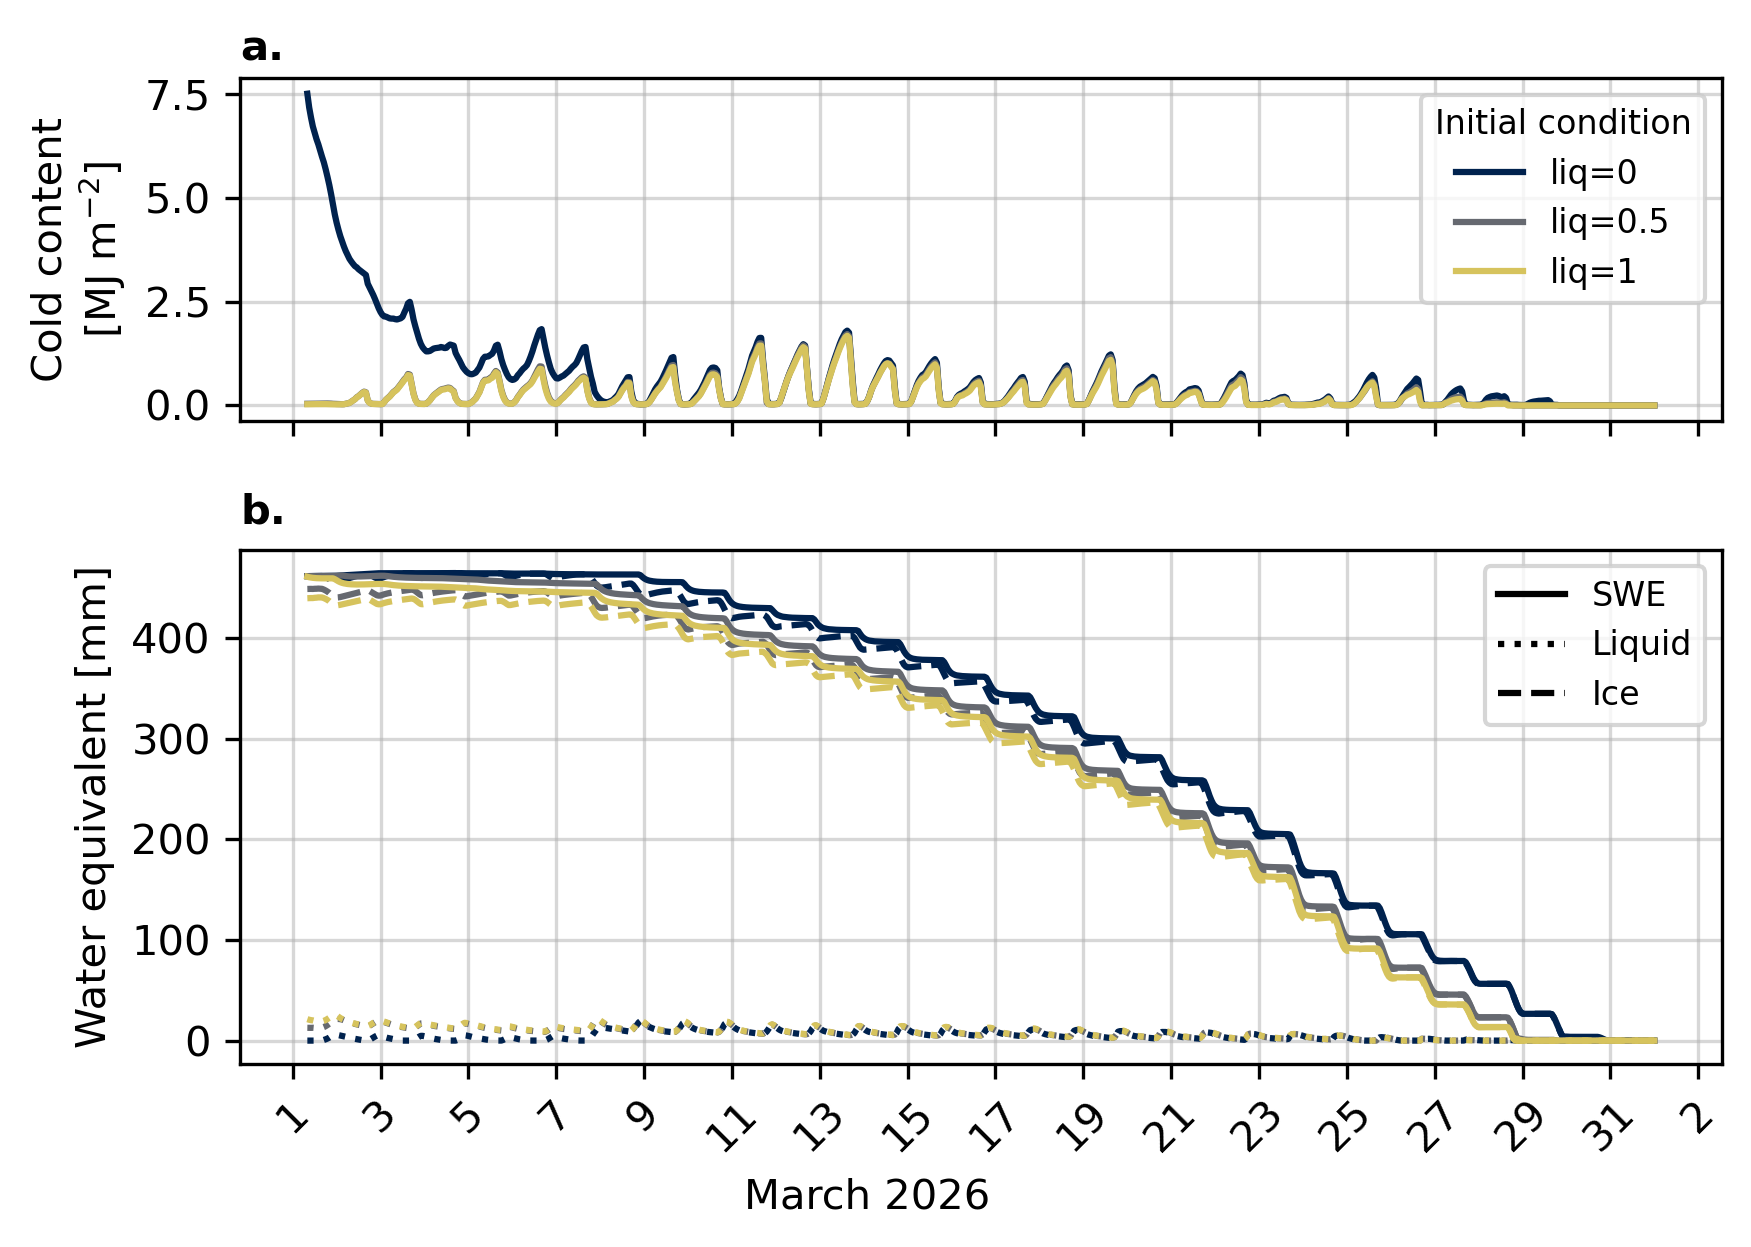
\includegraphics{images2/supp_initial_cond_sens_liq_and_CC.png}
  \caption{Initial condition Test 1: Effects of liquid water content. (a) shows the hourly CC of the snowpack throughout the model run. (b) Depicts the total SWE, liquid water content, and ice water equivalent integrated throughout the depth of the pack in units of water equivalent (mm).}
  \label{fig:supp_initial_cond_sens1}
\end{figure}

\begin{figure}[htbp]
  \centering
  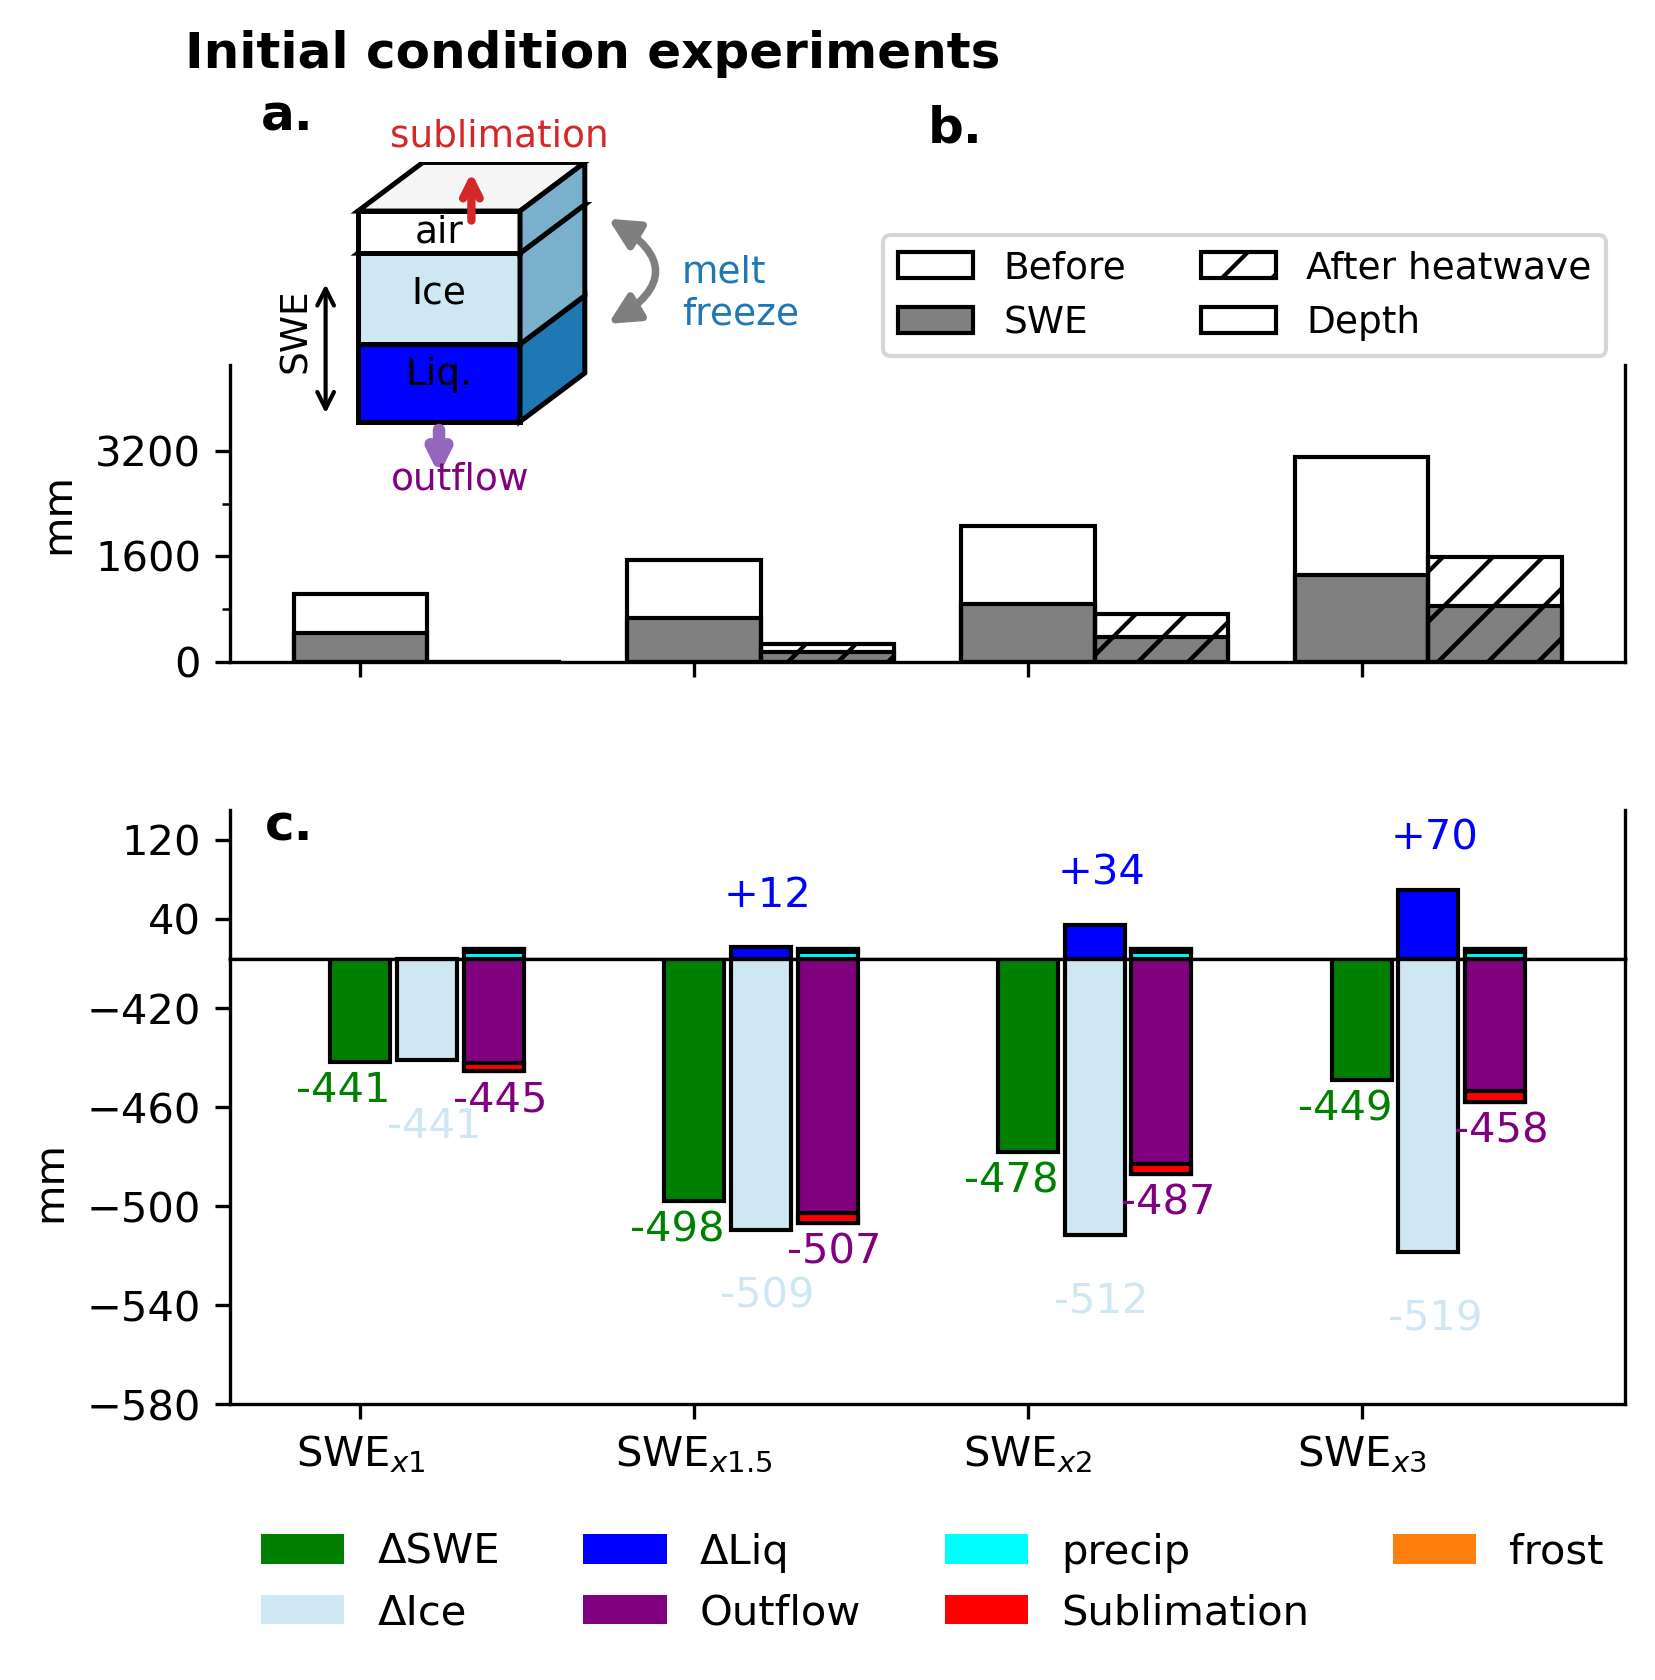
\includegraphics{images2/initial_cond_sens.png}
  \caption{Initial condition Test 2: effects of dry snow amount. (a) Depicts the initial and final SWE and snow depth (starting on March 1 and ending on March 31) for the four experiments.
  (b) Depicts mass components of the change in SWE for the different experiments.
  Text lists $\Delta$SWE, $\Delta$Ice, $\Delta$Liq, and total Outflow, respectively.
  }
  \label{fig:supp_initial_cond_sens2}
\end{figure}

\end{document}
